\documentclass[tikz,border=10pt]{standalone}
% Shared look for every TikZ diagram. Load with % Shared look for every TikZ diagram. Load with % Shared look for every TikZ diagram. Load with \input{../../tools/tikz-style.tex}
\usepackage[T1]{fontenc}
\usepackage{lmodern}
\renewcommand{\sfdefault}{lmr}  % diagrams use the same serif as the text
\usetikzlibrary{arrows.meta, positioning, shapes.geometric, calc, fit, backgrounds}
\definecolor{cblue}{HTML}{4C78A8}
\definecolor{corange}{HTML}{F58518}
\definecolor{cgreen}{HTML}{54A24B}
\definecolor{cred}{HTML}{E45756}
\definecolor{cpurple}{HTML}{B279A2}
\definecolor{cgrey}{HTML}{6B6B6B}
\tikzset{
  every picture/.style={font=\sffamily, line width=1.2pt},
  box/.style={draw=#1, fill=#1!12, rounded corners=4pt, align=center, inner sep=7pt, minimum height=1.1cm},
  box/.default=cgrey,
  arrow/.style={-{Stealth[length=3mm]}, draw=cgrey, line width=1.4pt},
  title/.style={font=\sffamily\bfseries\Large},
  note/.style={font=\sffamily\small, text=cgrey, align=center},
}
\AtBeginDocument{\hyphenpenalty=10000 \exhyphenpenalty=10000}

\usepackage[T1]{fontenc}
\usepackage{lmodern}
\renewcommand{\sfdefault}{lmr}  % diagrams use the same serif as the text
\usetikzlibrary{arrows.meta, positioning, shapes.geometric, calc, fit, backgrounds}
\definecolor{cblue}{HTML}{4C78A8}
\definecolor{corange}{HTML}{F58518}
\definecolor{cgreen}{HTML}{54A24B}
\definecolor{cred}{HTML}{E45756}
\definecolor{cpurple}{HTML}{B279A2}
\definecolor{cgrey}{HTML}{6B6B6B}
\tikzset{
  every picture/.style={font=\sffamily, line width=1.2pt},
  box/.style={draw=#1, fill=#1!12, rounded corners=4pt, align=center, inner sep=7pt, minimum height=1.1cm},
  box/.default=cgrey,
  arrow/.style={-{Stealth[length=3mm]}, draw=cgrey, line width=1.4pt},
  title/.style={font=\sffamily\bfseries\Large},
  note/.style={font=\sffamily\small, text=cgrey, align=center},
}
\AtBeginDocument{\hyphenpenalty=10000 \exhyphenpenalty=10000}

\usepackage[T1]{fontenc}
\usepackage{lmodern}
\renewcommand{\sfdefault}{lmr}  % diagrams use the same serif as the text
\usetikzlibrary{arrows.meta, positioning, shapes.geometric, calc, fit, backgrounds}
\definecolor{cblue}{HTML}{4C78A8}
\definecolor{corange}{HTML}{F58518}
\definecolor{cgreen}{HTML}{54A24B}
\definecolor{cred}{HTML}{E45756}
\definecolor{cpurple}{HTML}{B279A2}
\definecolor{cgrey}{HTML}{6B6B6B}
\tikzset{
  every picture/.style={font=\sffamily, line width=1.2pt},
  box/.style={draw=#1, fill=#1!12, rounded corners=4pt, align=center, inner sep=7pt, minimum height=1.1cm},
  box/.default=cgrey,
  arrow/.style={-{Stealth[length=3mm]}, draw=cgrey, line width=1.4pt},
  title/.style={font=\sffamily\bfseries\Large},
  note/.style={font=\sffamily\small, text=cgrey, align=center},
}
\AtBeginDocument{\hyphenpenalty=10000 \exhyphenpenalty=10000}

\begin{document}
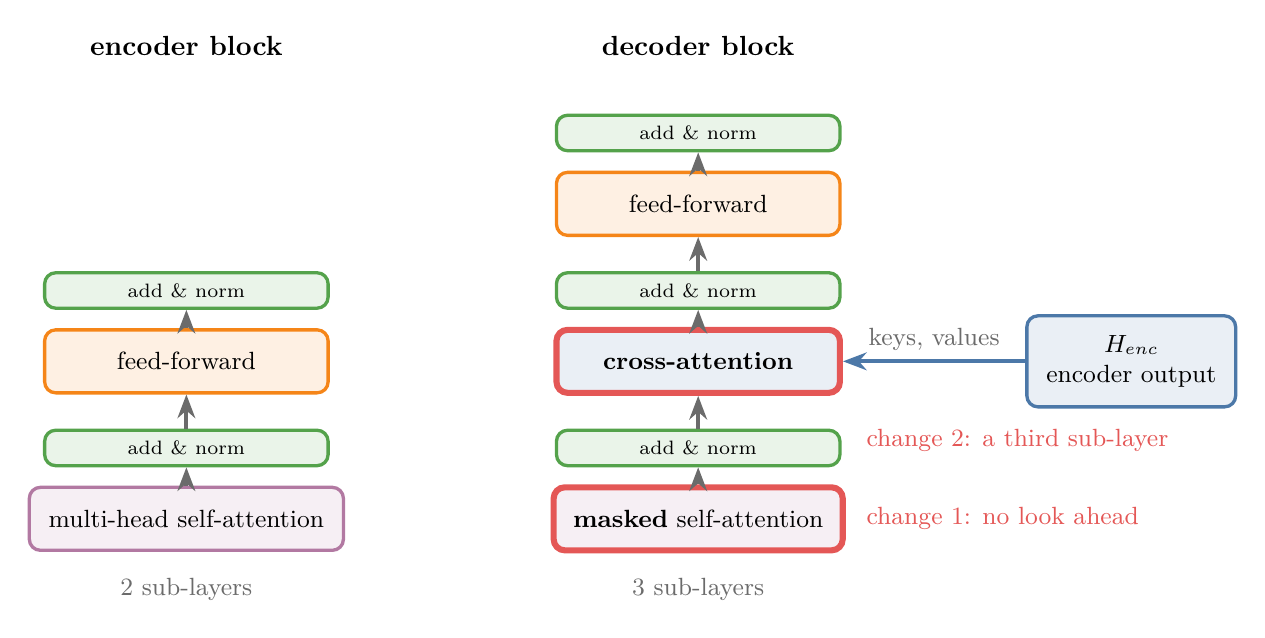
\begin{tikzpicture}[sl/.style={box=#1, minimum width=3.6cm, minimum height=0.8cm, font=\sffamily\small},
  an/.style={box=cgreen, minimum width=3.6cm, minimum height=0.45cm, inner sep=2pt, font=\sffamily\scriptsize}]
  \node[font=\sffamily\bfseries] at (0,6.6) {encoder block};
  \node[sl=cpurple] (a) at (0,0.6) {multi-head self-attention};
  \node[an] (n1) at (0,1.5) {add \& norm};
  \node[sl=corange] (f) at (0,2.6) {feed-forward};
  \node[an] (n2) at (0,3.5) {add \& norm};
  \draw[arrow] (a) -- (n1); \draw[arrow] (n1) -- (f); \draw[arrow] (f) -- (n2);
  \node[font=\sffamily\bfseries] at (6.5,6.6) {decoder block};
  \node[sl=cpurple, draw=cred, line width=2.2pt] (da) at (6.5,0.6) {\textbf{masked} self-attention};
  \node[an] (d1) at (6.5,1.5) {add \& norm};
  \node[sl=cblue, draw=cred, line width=2.2pt] (dc) at (6.5,2.6) {\textbf{cross-attention}};
  \node[an] (d2) at (6.5,3.5) {add \& norm};
  \node[sl=corange] (df) at (6.5,4.6) {feed-forward};
  \node[an] (d3) at (6.5,5.5) {add \& norm};
  \draw[arrow] (da) -- (d1); \draw[arrow] (d1) -- (dc); \draw[arrow] (dc) -- (d2); \draw[arrow] (d2) -- (df); \draw[arrow] (df) -- (d3);
  \node[box=cblue, font=\sffamily\small] (h) at (12.0,2.6) {$H_{\text{enc}}$\\encoder output};
  \draw[arrow, draw=cblue] (h) -- node[above, note] {keys, values} (dc);
  \node[note, text=cred, anchor=west] at (8.5,0.6) {change 1: no look ahead};
  \node[note, text=cred, anchor=west] at (8.5,1.6) {change 2: a third sub-layer};
  \node[note] at (0,-0.3) {2 sub-layers};
  \node[note] at (6.5,-0.3) {3 sub-layers};
\end{tikzpicture}
\end{document}
